Music is all around us. Everybody listens to it in a different way \cite{Cox2012a}, only a few actually create it. Creating music takes a lot of effort; making sure all notes and tones form some kind of harmony and melody, and that all harmonies and melodies form a coherent piece, among many other difficult aspects that involve creating music. Although these aspects are all very difficult and only some people are actually good at it, computers are far worse in it.\\
Listening to music involves many subconscious processes that are influenced by, among other things, emotion. Therefore making a computer understand the concept of music is a difficult task.
Due to the hierarchical properties of music \cite{Cooper1960rhythmic, Lerdahl1983overview}, one of the first steps of this process is understanding the musical structure of a piece of music. This will be the main focus of this thesis.


\section{Musical Structure}
The musical structure of a piece of music can be defined in many different ways; on a high level or low level, and can be of different meanings in different kinds of music.\\
Therefore for the remainder of this thesis I will refer to music as music in the genre of Western Popular Music \cite{Serra2012measuring} and make the following definitions:

\theoremstyle{definition}
\adddeftocontentsline{def:musical_structure}{Musical Structure}
\begin{theoremEnd}[restate,category=def]{defEnd}[Musical Structure]
    \label{def:musical_structure}
    The \textit{Musical Structure} of a piece of music is a series of \textit{segments} (\ref{def:segment}) that describes the high-level structure of a piece of music.
\end{theoremEnd}

\adddeftocontentsline{def:segment}{Segment}
\begin{theoremEnd}[restate,category=def]{defEnd}[Segment]
    \label{def:segment}
    A \textit{Segment} is one consecutive piece of audio in a piece of music that has one \textit{segment function} (\ref{def:segment_function}), with a start- and an end-boundary.
\end{theoremEnd}

\adddeftocontentsline{def:segment_function}{Segment Function}
\begin{theoremEnd}[restate,category=def]{defEnd}[Segment Function]
    \label{def:segment_function}
    Following the definitions as they can be found in \textcite{Benward1997music}, Part B: \textit{The Structural Elements of Music}, a \textit{Segment Function} is the function of a \textit{segment}, this is either:
    \begin{itemize}[noitemsep]
        \item Chorus
        \item Verse
        \item Bridge
        \item Interlude / Transition
        \item Intro
        \item Outro
        \item Solo
        \item (Silence)
        \item (Background Noise)
    \end{itemize}
\end{theoremEnd}

I will refer to the extraction of the musical structure of a piece of music as \textit{Musical Structure Analysis} or MSA. An example of musical structures can be found in \autoref{fig:music_structures_examples}. The aim of this thesis is to produce a structure of a song similar to \ref{fig:music_structures_examples}e and \ref{fig:music_structures_examples}f, where \textbf{I} stands for intro, \textbf{V1} stands for Verse 1, etc.

\begin{figure}[t]
    \centering
    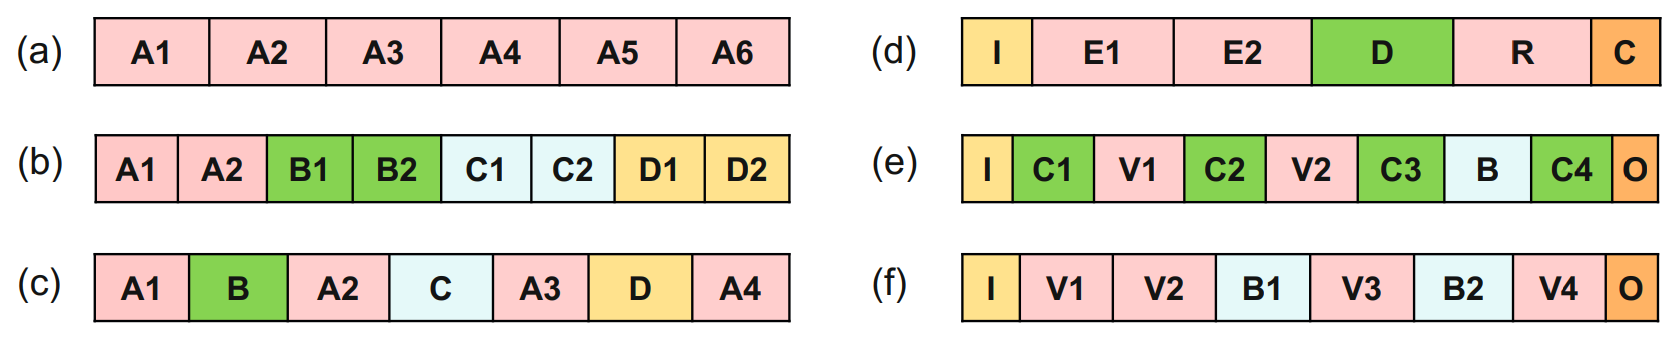
\includegraphics[width=1\textwidth]{images/music_structures_examples}
    \caption{Examples for musical structures as encountered in Western music. \textbf{(a)} Strophic form. \textbf{(b)} Chain form with repetitions. \textbf{(c)} Rondo form. \textbf{(d)} Sonata form. \textbf{(e)} Beatles song “Tell Me Why.” \textbf{(f)} Beatles song “Yesterday.”\\
    Reprinted from \textcite[p. 173]{Muller} (Figure 4.4)}
    \label{fig:music_structures_examples}
\end{figure}


\section{Applications}
The musical structure of a piece of music has many applications, within research and the industry. For example the musical structure can be used to only retrieve a certain part of a piece of music. This can then be used to preview only the chorus of a song when someone is browsing through a list of songs to find a certain song. Being able to quickly seek through a song to its verses or chorus can be of great addition to many music streaming, or other streaming, services. 

More commercial applications could be to limit ones listening capabilities by restricting a user to listen only to the verse or chorus of a song, while blocking the other parts of a song behind some pay-wall. Less aggressive commercial applications could be to place an advert between for example the verse and chorus, when the user is using a free subscription to a music streaming service.

The scope of this thesis, however, will be to place the music structure problem in a more research driven, less commercial field, and the field of AI in particular.

\subsection{Relevance to AI}
Finding and analyzing the structure of a musical piece is an important part of music information retrieval and an important step in music processing and music analysis, both for humans and computers. Once an understanding of the basic structure of a piece of music is established, it can be used to establish more complex understandings about that piece of music.

One of these uses may be to use the musical structure to get more insight in how certain songs are equal to each other, or how certain structures are used for certain kinds of songs or in certain genres. This thus may be used as additional information when finding for example the genre of a piece of music.

Another way of using this musical structure could be to extract lower level musical patterns from a piece of music. This could be leading melodies, a riff\footnote{A famous example of a (rock) riff can be found in \textit{Smoke on the Water} played by Ritchie Blackmore of Deep Purple.}, lyrics or the hook \cite{Covach2005form} of a song \cite{Chai2005automated}.

Additionally, knowledge about the structure of songs that are produced by humans can be used for generating songs using computers. This information can for example be used as additional information during the generation phase, or as validation information for already generated songs to validate whether these generated songs comply to human musical structure.\\

For humans, finding the musical structure is quite trivial, because they constantly and often unconsciously adapt themselves to the musical and acoustic properties of what they listen to. However the amount of different musical structures make computational structure analysis a challenging problem.


\section[SbA vs DSA]{\sba\ versus\\ \dsa}
Extracting the musical structure of a piece of music can be done in a few ways, however almost all of these methods can be generalized into two general approaches: \textit{\sba}\ (SbA) and \textit{\dsa} (DSA).

\adddeftocontentsline{def:SbA}{\sba}
\begin{theoremEnd}[restate,category=def]{defEnd}[\sba]
    \label{def:SbA}
    \textbf{\sba} in the context of music structure analysis means first dividing a song into many small pieces (e.g. pieces of 10ms or every beat). Thereafter a \textit{segment function} is assigned to each small piece using some kind of classification method (e.g. statistics, support vector machine, deep learning). Sequences of similarly annotated small pieces are then combined into \textit{segments}, resulting in the musical structure of the song.
\end{theoremEnd}

\adddeftocontentsline{def:DSA}{\dsa}
\begin{theoremEnd}[restate,category=def]{defEnd}[\dsa]
    \label{def:DSA}
    \textbf{\dsa} in the context of music structure analysis means first finding segment boundaries using some kind of distance metric. Subsequently these segments are grouped into groups that are similar to each other in their structural role in the piece of music, using some kind of grouping method (e.g. nearest neighbors, support vector machines), resulting in each segment getting a capital letter denoting their function. Then, each capital letter is converted into a segment function, this can be either done using some kind of statistics, pattern matching or machine learning method.
\end{theoremEnd} 

\dsa\ has been researched a lot in the context of music structure analysis and was for a long time the best approach. See \autoref{ch:r_work} for an overview of research in this areas. \sba\ has been used a lot less for this exact application but more for separating and classifying pieces of speech, music and different kind of background noises in an audio stream. This is because speech, music and background noise all differ a lot more in their auditory features than different parts of music within the same piece. Because the use of the distance-based approach yielded increasingly better results, recent research focused on that. However with the increasing popularity and performance of machine learning in many disciplines like computer vision or natural language processing and production, applying machine learning to the music structure problem has become increasingly popular.


\section{Combined Research}
Although the DSA approach to MSA is become state-of-the-art, its results can always be improved. Therefore not only putting effort into improving the \sba\ approach but also the \dsa\ approach will benefit the \msa\ problem. This work is related to \textcite{Jesperthesis} in such a way that this work focuses on the \sba\ approach, and \citeauthor{Jesperthesis} focuses on giving an overview and improvement of the \dsa\ approach.


\section{Research Questions}
The following research questions can be formulated:

\addrqtocontentsline{rq:main}
\begin{theoremEnd}[restate,category=rq]{rqEnd}[Main RQ]
    \label{rq:main}
    What is the feasibility of a machine learning implementation of the \sba\ approach to \msa\ in Western Popular Music?
\end{theoremEnd}

The sub-questions that are part of this main research question are:

\addrqtocontentsline{rq:sub1}
\begin{theoremEnd}[restate,category=rq]{rqEnd}[Sub-RQ 1]
    \label{rq:sub1}
    Which deep learning architecture, implementing the \sba\ approach to \msa, yields the best relative results?
\end{theoremEnd}

\addrqtocontentsline{rq:sub2}
\begin{theoremEnd}[restate,category=rq]{rqEnd}[Sub-RQ 2]
    \label{rq:sub2}
    How does the performance of the best performing deep learning architecture, implementing the \sba\ approach to \msa, compare to the performance of implementations of the \dsa\ approach, and a state-of-the-art implementation in particular?
\end{theoremEnd}

To answer the main research question I will create different types of deep learning models, using different kinds of architectures. Then I will train these models on different combinations of musical features extracted from the songs present in the internet archives subset of the SALAMI dataset (see \autoref{sec:3.the_data} for an explanation of this dataset). I will use the annotations, produced by human annotators, of these songs as ground truth to determine the absolute performance of each implementation. The absolute performance of the best performing implementation can then be used to compare a machine learning application of the \sba\ approach to MSA to the absolute performance of a state-of-the-art implementation of the \dsa\ approach, determined in the same way. I will elaborate more on this in \autoref{ch:method}.


\section{Outline}
In \autoref{ch:r_work} I will first explore previous work regarding the SbA and DSA approach. Here I will also discuss the current state-of-the-art and describe the background of the models I created. Lastly I will give an overview of the dataset I used, and a listing of possible acoustic features that can be extracted from this dataset.

In \autoref{ch:method} I introduce the architectures of the models I created. In this chapter I also describe the data preparation and feature selection that preceded the testing phase of this research.

Then, in \autoref{ch:results} I describe the training and evaluation setup and some preliminary results. A final test setup is described as well as the final results following from this final test.

Thereafter, \autoref{ch:discussion} discusses these results and explores reasons for these results. It concludes with a comparison between the segmentation by annotation approach and distance-based segmentation and annotation approach to music structure analysis.

This thesis ends with \autoref{ch:future_research}. In this final chapter I propose future research that can be performed to improve both the segmentation by annotation approach to music structure analysis as well as music structure analysis in general. This chapter ends with an comparison of machine learning versus symbolic approaches to music structure analysis as well as artificial intelligence problems in general.